
\documentclass[12pt]{article}
\usepackage{graphicx}
\usepackage[utf8]{inputenc}
\usepackage[nottoc]{tocbibind}
\usepackage{graphicx}
\usepackage{wrapfig}
 \usepackage{url}


\begin{document}


%===================================TTLE PAGE===================================%		
	\title{Differential Equations for the Growth of Coral Polyps of the Genus \textit{Acropora}}
	\author{Kyle Spooner, Ethan Puerto, and Holly Pafford}
	\maketitle
	\newpage

%===================================CONTENTS====================================%		
	\tableofcontents
	\newpage
	
%===================================ABSTRACT====================================%	
	\section{Abstract}
		Coral farming and propagation is necessary due the decline in coral reef habitats around the world. One the Caribbean's most ``predominant reef-building coral'' genera, \textit{Acropora}, is also facing the same problem. This has resulted in a decrease of reef function which in turn causes widespread oceanic population decline. In the propagation of \textit{Acropora}, the polyp population can be estimated by a simple exponential growth differential equation model. We will analyze the exponential growth of these polyps using the relationship of the number of starting polyps and time, with this information we can estimate coral regeneration rates.
	\newpage
	
	\section{Introduction}


	
	Oceans cover approximately 71 percent of the Earth’s surface. Within these bodies of water, coral reefs exist. Reefs are key to developing new types of medications for curing infections, diseases, and even cancer. In addition to that, reefs have been a major food source for millions across the globe for eons. The reef ecosystem is vital to the ocean as a whole, it is part of every food chain and is the backbone for all life in the ocean. Reefs are the product of millions of years of growth and development, the reefs we see and rely on today are built on Acropora from the past.\cite{wiki:Acropora}
	

	
	
	\begin{wrapfigure}{r}{0.6\textwidth}
		\begin{center}
			\includegraphics[width=0.48\textwidth]{acroplate}
		\end{center}
		\caption{Branching Plate \textit{Acropora}\cite{wiki:Acropora}}
	\end{wrapfigure}
	
	
	 \textit{Acropora} is defined as a ``small polyp stony coral''. This genus, in particular, is responsible for building the calcium carbonate substructure that helps to support the frame of a reef ecosystem. Approximately 149 species of \textit{Acropora} has been identified. These species can come in a variety of forms, such as plates and branches. All \textit{Acropora} corals are essentially colonies of many individual polyps that have the ability to withdraw back into their hard exoskeleton as a response to sudden movement in the area which may be a potential predator. Recently, there has been a population decline caused by environmental destruction; therefore, propagation of \textit{Acropora} is necessary to keep reef ecosystems alive.\cite{wiki:Acropora}
	 
	
	
	\subsection{\textit{Acropora} Growth Through Propagation}
	
	Propagation is when a small fragment of coral is taken from a much larger colony. This fragment, or frag, then reproduces asexually resulting a large colony of its own. Multiple methods exist for propagating coral. These methods are divided into one of two types, “floating” propagation or “fixed to the bottom” propagation. In floating propagation,the coral frag is tethered to a line above the ocean floor. In this case, coral is capable of growing in any direction due to being suspended in the water column. In fixed to the bottom propagation, frags are attached to ceramic plugs, cinder blocks, or various other materials and placed on what is essentially a table. In this placement the coral growth is limited to upwards and outwards growth. By using these methods we can help stimulate the growth of coral colonies and aid in the restoration of coral reefs.\cite{GrowthDynamics}
	
	\begin{figure}[h]
		\centering
		\includegraphics[width=0.6\textwidth]{acroprop}
		\caption{Propogation methods for \textit{Acropora}\cite{GrowthDynamics}}
	\end{figure}
	



%==================================CONTENT======================================%		

	\section{The Equation for Modeling Polyp Growth}
	In order to properly model the growth of these polyps we must first take into account the various aspects of this problem. With the growth of \textit{Acropora}, or any animal for that matter, we must understand its growth rate and factor that into our solution. In addition to that, time, and starting population are necessary to allow for a broad a general solution and model.
	
	The differential equation that results is the same used to model most exponentially growing population\cite{BaseFunction},
	
	\begin{equation}
		\frac{dy}{dt} = ky
	\end{equation}

	
	Rearanging the equation allows it to be integrated on each side with respects to $y$ and $t$
	
	\begin{equation}
		\frac{1}{y}\frac{dy}{dt}=k
	\end{equation}
	
	From this point we must manipulate the equations to allow for a clean integration of boths sides in terms of $dy$ on the left and $dt$ on the left.
	
	\begin{equation}
		\frac{1}{y}dy=kdt
	\end{equation}
	
	Now we can integrate both sides with there own respects.
	
	\begin{equation}
		\int{\frac{1}{y}}dy = \int {k}dt
	\end{equation}
	
	Since we know the integral of $\frac{1}{y}$ with respects to $y$ and the integral of a constant $k$, we can derive the following solution.
	
	\begin{equation}
		ln(y)= kt+c
	\end{equation}
	
	For the final step in deriving the solution we must isolate $y$. Using log rules we can remove $ln()$ from $ln(y)$.
	
	\begin{equation}
		y=Ce^{kt}
	\end{equation}
	
		At this point, the equation can be used to model any species of coral. Sample data, including a starting number of polyps, end number of polyps, and time between would be used to determine the rate constant k.
	
	
	 This equation also resembles the Malthusian Growth Model.
	

	\subsection{Malthusian Growth Model}	
	
	This model is used to represent the growth of various populations over a generally short period of time. This is due to the simple exponential properties of this equation which results in an infinite solution, when in reality it is never as such.\cite{wiki:Equation} The equation is as follows,
	
	\begin{equation}
		P(t)= P_{0}e^{rt}
	\end{equation}
	
	Where,
	\begin{itemize}
		\item $P_{0}$ is the initial population size
		\item $r$ is the growth rate
		\item $t$ is the length of time
	\end{itemize}

	\section{Modeling Growth using the Solution}
	\subsection{Solving for $P(t)$}
	A Staghorn Coral (\textit{Acropora cervicornis}) of length $10cm$ can grow up to $200mm$ in its first year. With an average number of polyps per linear millimeter of \textit{Acropora} being $10$, we can find the rate constant for this species.\cite{AcroStats}
	
	First we must find the starting polyps for $10cm$ of coral,
	\begin{equation}
		100mm*10=1000
	\end{equation}
	
	Using this, we can also find the final population after a year knowing that \textit{Acropora Staghorn} grows at a race of 200mm per year.
	\begin{equation}
		P(t)=1000+2000=3000
	\end{equation}
	
	\subsection{Finding the Growth Rate Constant $k$}
	Now by substituting in the values of $P(t)$,$P_{0}$, and $t=1$; we can solve for our growth rate $k$
	
	\begin{equation}
		3000 = 1000e^{k(1)}
	\end{equation}
	
	\begin{equation}
		3=1e^{k}
	\end{equation}
	
	\begin{equation}
		ln3=k
	\end{equation}
	
	\begin{equation}
		k=1.0986
	\end{equation}
	
	\subsection{Growth Estimation}
	We can now use this information to estimate the length of staghorn coral for various periods of time.
	For example, a coral containing 500 polyps that grows under ideal conditions for 5 years would reach a population of:
	
	\begin{equation}
		P = 500e^{1.0986(5)} = 12,150
	\end{equation}
	
	This resultant coral of 12,150 polyps, would have a length of 
	
	\begin{equation}
		\frac{12150 Polyps}{10 Polyps Per Millimeter} =1125mm=1.25m
	\end{equation}
	
	\textit{(This length is the overall tip to tail length of all branches added together, not of each branch.) }
	
	The average length of a branch of staghorn is $10cm$\cite{AcroStats}. With this we can also solve for the final number of branches.
	
	\begin{equation}
		\frac{1.25m}{10cm}=11.25
	\end{equation}
	
	Finding the changes in number of polyps in a coral allows us to gather a variety of information on the coral, including estimations in length, growth rate and branch production. This same process can be applied to any species of the genus acropora, as long as experimental data can be supplied to determine the rate constant.
	
	\newpage
	
	\subsection{Matlab Estimation}
	The estimation of equation 14 in matlab is as follows,
	
	\begin{center}
		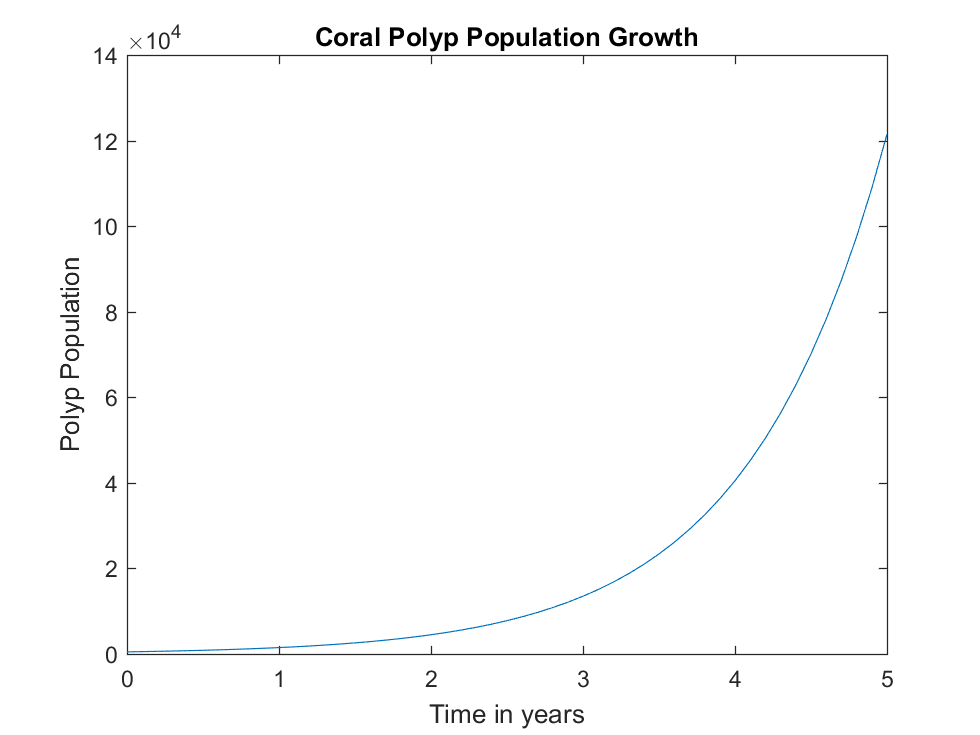
\includegraphics[width=1\textwidth]{PolypPopGrowth}
	\end{center}
	
	\newpage

	\section{Conclusion}
	Exponential growth is a great way for estimating the time at which a particular species needs to re-populate itself. For example, \textit{Acropora} is not re-populating itself fast enough for the survival of reef habitats; therefore, propagation of \textit{Acropora} must take place. The chosen differential equation and derived solution is necessary for the estimated growth rate of A\textit{Acropora} (i.e. Staghorn). The equation may be used for estimating the growth rate of any coral genus; however, the constant(s) must be altered according to the specific species. The solution allows the researcher to alter the coral’s environment to reach full production.    
	



	\newpage
	\bibliographystyle{plain}
-	\bibliography{bib}
	

	
	
\end{document}